\chapter{Related Work}\label{cap:relatedWork}

Ao decorrer desse capitulo será abordado uma breve revisão bibliográfica para que o leitor possa ter um conhecimento mínimo a respeito dos temas abordados. Na secção \ref{sec:smartFactories}, será debatido sobre \emph{"Smart Factories"}: origem do tema, avanços na área e desafios. 


\section{Smart Factories}
\label{sec:smartFactories}

Especialistas alemães formaram o conceito de Industria 4.0 para promover uma nova revolução industrial \cite{Grabowska+2020+90+96}. Esta abordagem visa promover uma nova geração de instalações de fabricação que utilizem tecnologias avançadas para otimizar a manufatura e o controle de processos em tempo real. Países da União Europeia adotaram esse modelo para melhorar o aproveitamento de recursos naturais e aumentar a competitividade de suas indústrias, especialmente diante da transferência gradual de seu protagonismo industrial para países emergentes.

O conceito de  \emph{"Smart Factory"} iniciou-se em regiões industrializadas. Os países europeus foram  pioneiros em desenvolver esse novo conceito de indústria, em especial, a Alemanha, a qual cunhou o termo Industria 4.0 em 2011 \cite{Grabowska+2020+90+96}. Nos últimos anos, a queda da competitividade no setor industrial desses países por questões de baixa natalidade ou altos salários, fez com que esses adotassem uma estratégia industrial liderada pelo o uso de tecnologias como: robôs, sensores, Big Data, machine learning, deep learning , \acrfull{iiot}, \acrfull{ai}, analise de dados e redes de telecomunicação entre dispositivos \cite{HerreroMeasuringTheEffectivenessOfIndustrialProcesses}. Por esse motivo, essas regiões viram em uma maior automatização da indústria a oportunidade de suprir a carência por trabalhadores especializados e a necessidade de contrabalancear os  salários autos dos trabalhadores ativos com os custos de produção.  

Esse novo paradigma de industrialização está se torando cada vez mais importante para as empresas nos últimos anos. Para \textcite{Grabowska+2020+90+96}, é esperado que a implementação de tecnologias modernas e novas técnicas de gerenciamento alinhadas com a industria 4.0 tomarão conta da maior parte dos processos de manufatura nos próximos anos. A utilização de \acrshort{ai} faz parte desses novos artifícios que ganharam espaço na industria recentemente. Segundo \textcite{PeresIASmartFactory} os tópicos envolvendo \emph{deep learning} relacionados com o meio industrial que recentemente apresentaram maior interesse de pesquisa foram: optimização de energia, manutenção preditiva e controle de qualidade. Além disso, atualmente, houve grandes avanços em automatização de processos que envolvem tomada de decisão, supervisão de operações, serviços de manutenção e sistemas de segurança \cite{KUMAR2022121284}. Dessa forma, as inovações proporcionadas por uma industria mais voltada para a tecnologia ganham cada vez mais importância, pois possibilitam melhorar a eficiência, reduzir o desperdício e os erros e aumentar a produtividade.

Essa nova forma de industrialização traz novas características para a cadeia produtiva. A exemplo,  o aprofundamento da digitalização da industria para além do gerenciamento. Com a criação de  \emph{"smart products"}. Esses são produtos que estão integradas na cadeia de valor e fazem parte do ambiente virtual da empresa. Dessa forma, é possível saber sua localização no chão de fábrica, em que processo de produção esse está e, ainda, prover essas informações para que o cliente tenha acontecimento a respeito do seu pedido \cite{economies6030046}.

Outro ponto chave importante é que esse tipo de tecnologia pode ajudar corporações é na melhora da experiência dos usuários envolvidos na manufatar do produto quanto no seu consumo.  O uso de um sistema IIoT permite uma melhora de experiência tanto para o consumidor que seria o usuário final quanto para a equipe de desenvolvimento do produto \cite{Grabowska+2020+90+96}. Do ponto de vista do usuário final, a comunicação M2M pode permitir que o cliente rastreie em tempo real o estado de desenvolvimento do seu produto personalizado. Isso pode ser feito através da coleta de dados em tempo real sobre o processo produtivo e a disponibilização desses dados para o cliente através de um portal ou aplicativo. Isso pode proporcionar ao cliente uma visão mais clara do andamento do seu pedido e aumentar a satisfação com o serviço. Do ponto de vista da equipe de desenvolvimento do produto, a comunicação M2M pode permitir que os profissionais obtenham informações rapidamente sobre produtos anteriores com características semelhantes ao produto que estaria sendo desenvolvido. Isso pode ser feito através da coleta de atributos como informações geométricas, material, tempo de execução etc. Isso pode ajudar a equipe a entender melhor as necessidades e preferências dos clientes e agilizar o processo de modelação através da reutilização de projetos antigos.

No entanto, segundo \textcite{Gilchrist2016}, \emph{"smart factories"} não é um conceito futurístico. Essa forma de visão está presente na forma de produção atual e de décadas passadas. Por exemplo,  a fabricação de um carro envolve a soldagem de peças, a qual pode ser feita por \emph{"smart machines"} que são programadas para realizar esse trabalho com uma enorme precisão. No entanto, apesar de um processo especifico ser comum a vários modelos diferentes de automóveis, outros processos tendem a ser diferente para caracterizar um produto como sendo distinto do outro. Nesse modelo de produção, as partes dos automóveis podem ser deslocadas para setores diferentes da fábrica e rastreadas para obterem as suas devidas customizações. Essa maior maleabilidade de produção permite que uma única linha de produção seja capaz de produzir produtos com diferentes aspectos.

As indústrias 4.0 apresentam uma flexibilidade maior entre seus processos devido a possibilidade de uma interação maior entre sistemas cibernéticos e físicos \cite{Gilchrist2016}. Na indústria 3.0 é comum o uso de  \acrfull{erp} para o planejamento da execução dos processo de manufatura, além do uso de um sistema de software comumente denominado \acrfull{mes}, o qual cumpre o papel de gerenciar da execução das tarefas anteriormente planejadas, como pode ser observado na figura \ref{fig:erp}. Tal abordagem, além de não permitir uma maior maleabilidade de produção, possui outro problema: a rigidez entre os processos. Ou seja, caso haja uma falha de execução em uma determinada parte da linha produtiva é bem provável que todo o sistema seja afetado pois as partes estão rigidamente interligadas. Dessa forma, as \emph{"smart factories"} trazem o uso de \acrfull{cps}, esses sistemas são formados por softwares, sensores, atuadores e caso necessário uma interface de comando. A vantagem desse sitema é a possibildiade de monitoramento em tempo real da linha de produção e a flexibilidade na tomada de decisões.
\begin{figure}[h!]
    \centering
    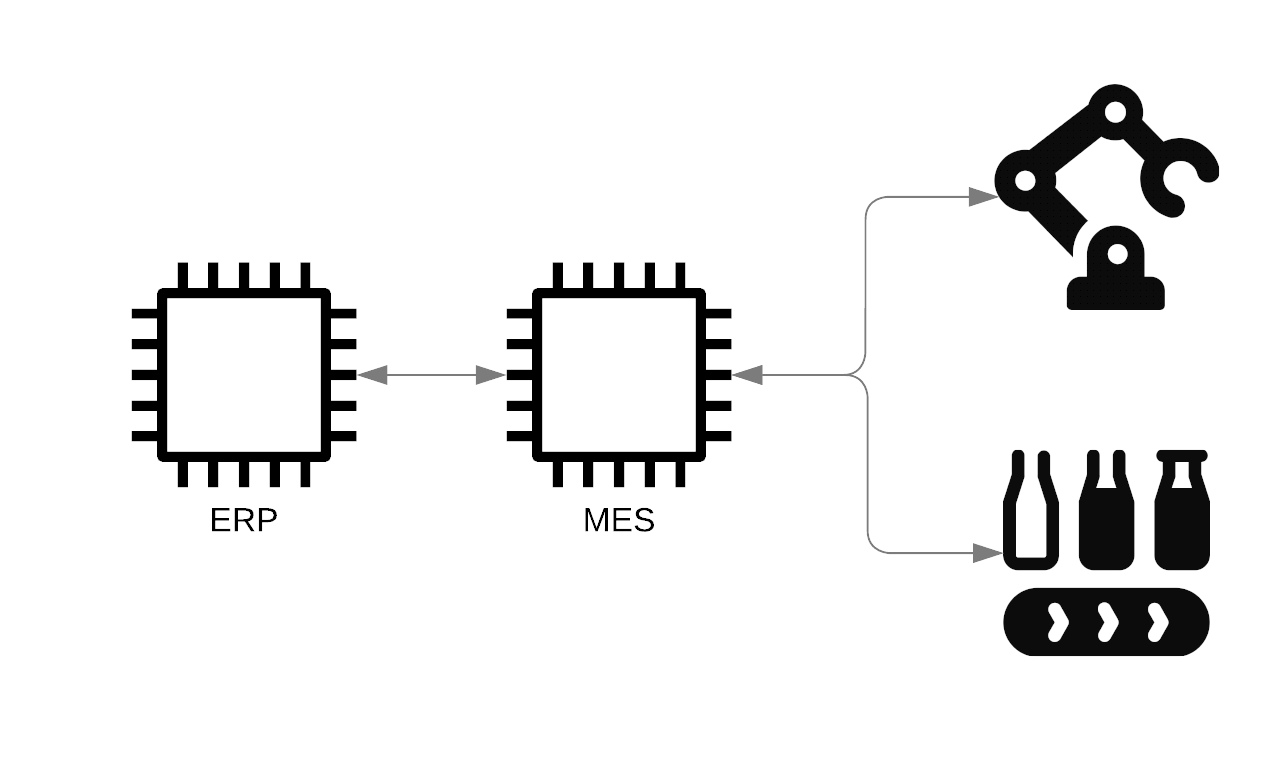
\includegraphics[scale=0.2]{images/Related/ERP.png}
    \caption{Common form of resource planning and management found in Industry 3.0 models. Source: adapted from \cite{Gilchrist2016}.}

    \label{fig:erp}
\end{figure}

O uso de \acrshort{cps} permite uma maior flexibilidade nas linhas de produção. Esses novos sistemas são mais responsivas as condições de fábrica. Ou seja, caso haja algum problema de produção ou alguma modificação seja necessária de ser realizado em um determinado produto, a linha de produção pode responder de forma quase que instantânea \cite{Gilchrist2016}. Por exemplo, caso haja uma peça faltando em uma esteira de linha de produção ou algum produto com defeito, o sistema pode avisar rapidamente que há um problema e, além disso, é possível que de forma automática ou não tome uma atitude para mitigar as conseqüências dessa falha. Essa é uma das razões para esse sistema ser mais flexível. Pois com o uso de \acrshort{cps} o sistema \acrshort{erp} pode acompanha a linha de produção quase que instantaneamente. O que da início há um novo tipo de software, os \acrfull{serp}.

\begin{figure}[h!]
    \centering
    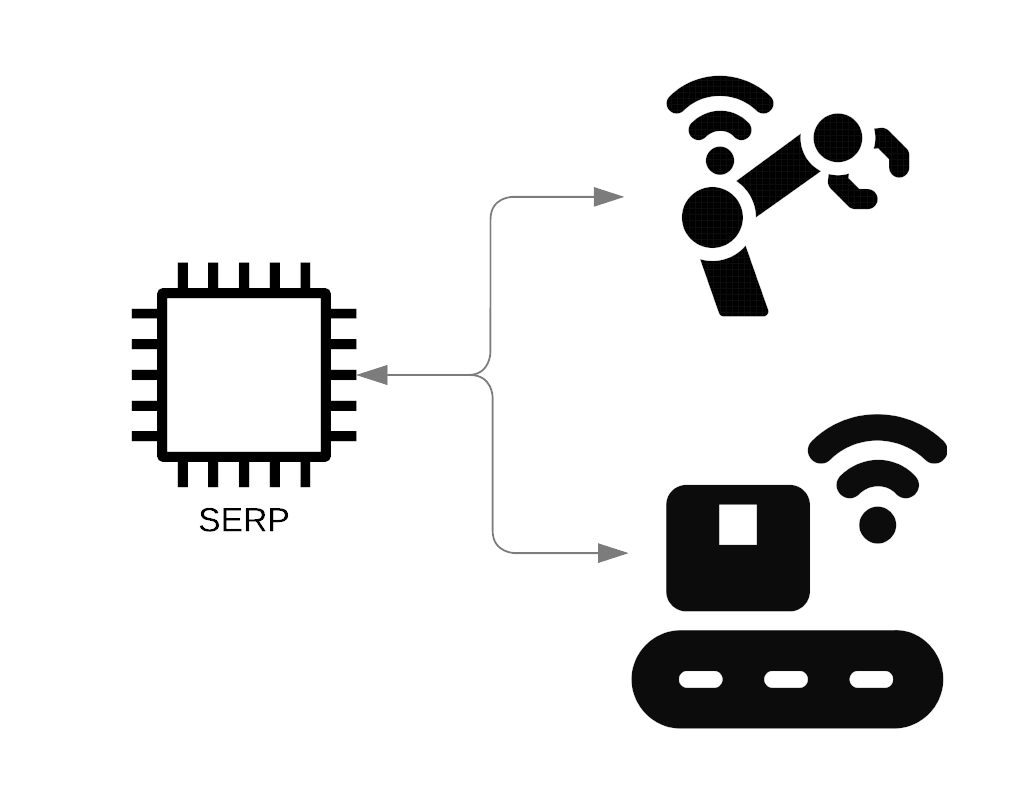
\includegraphics[scale=0.2]{images/Related/SERP.png}
    \caption{New form of resource planning and management found in Industry 4.0 models. Source: adapted from \cite{Gilchrist2016}.}

    \label{fig:serp}
\end{figure}

Os principais desafios encontrados na implementação de uma indústria 4.0 são divididos em duas partes: gerenciamento da  das novas tecnologias implementadas e desafios técnicos específicos de cada tecnologia envolvida. Por exemplo, o primeiro desafio está relacionado com a falta de recursos financeiros, pessoas capacitadas, falta de segurança ou entendimento das tecnologias. O segundo desafio tange os desafios relacionados a conectividade entre as tecnologias, por exemplo, interfaces de comunicação entre softwares específicos, infraestrutura de conectividade, desafio de criação de softwares, complexidade e etc. Esses dois ramos são os principais desafios para colocar em prática esse novo modelo de indústria \cite{Rikalovic2022}.

\begin{figure}[h!]
    \centering
    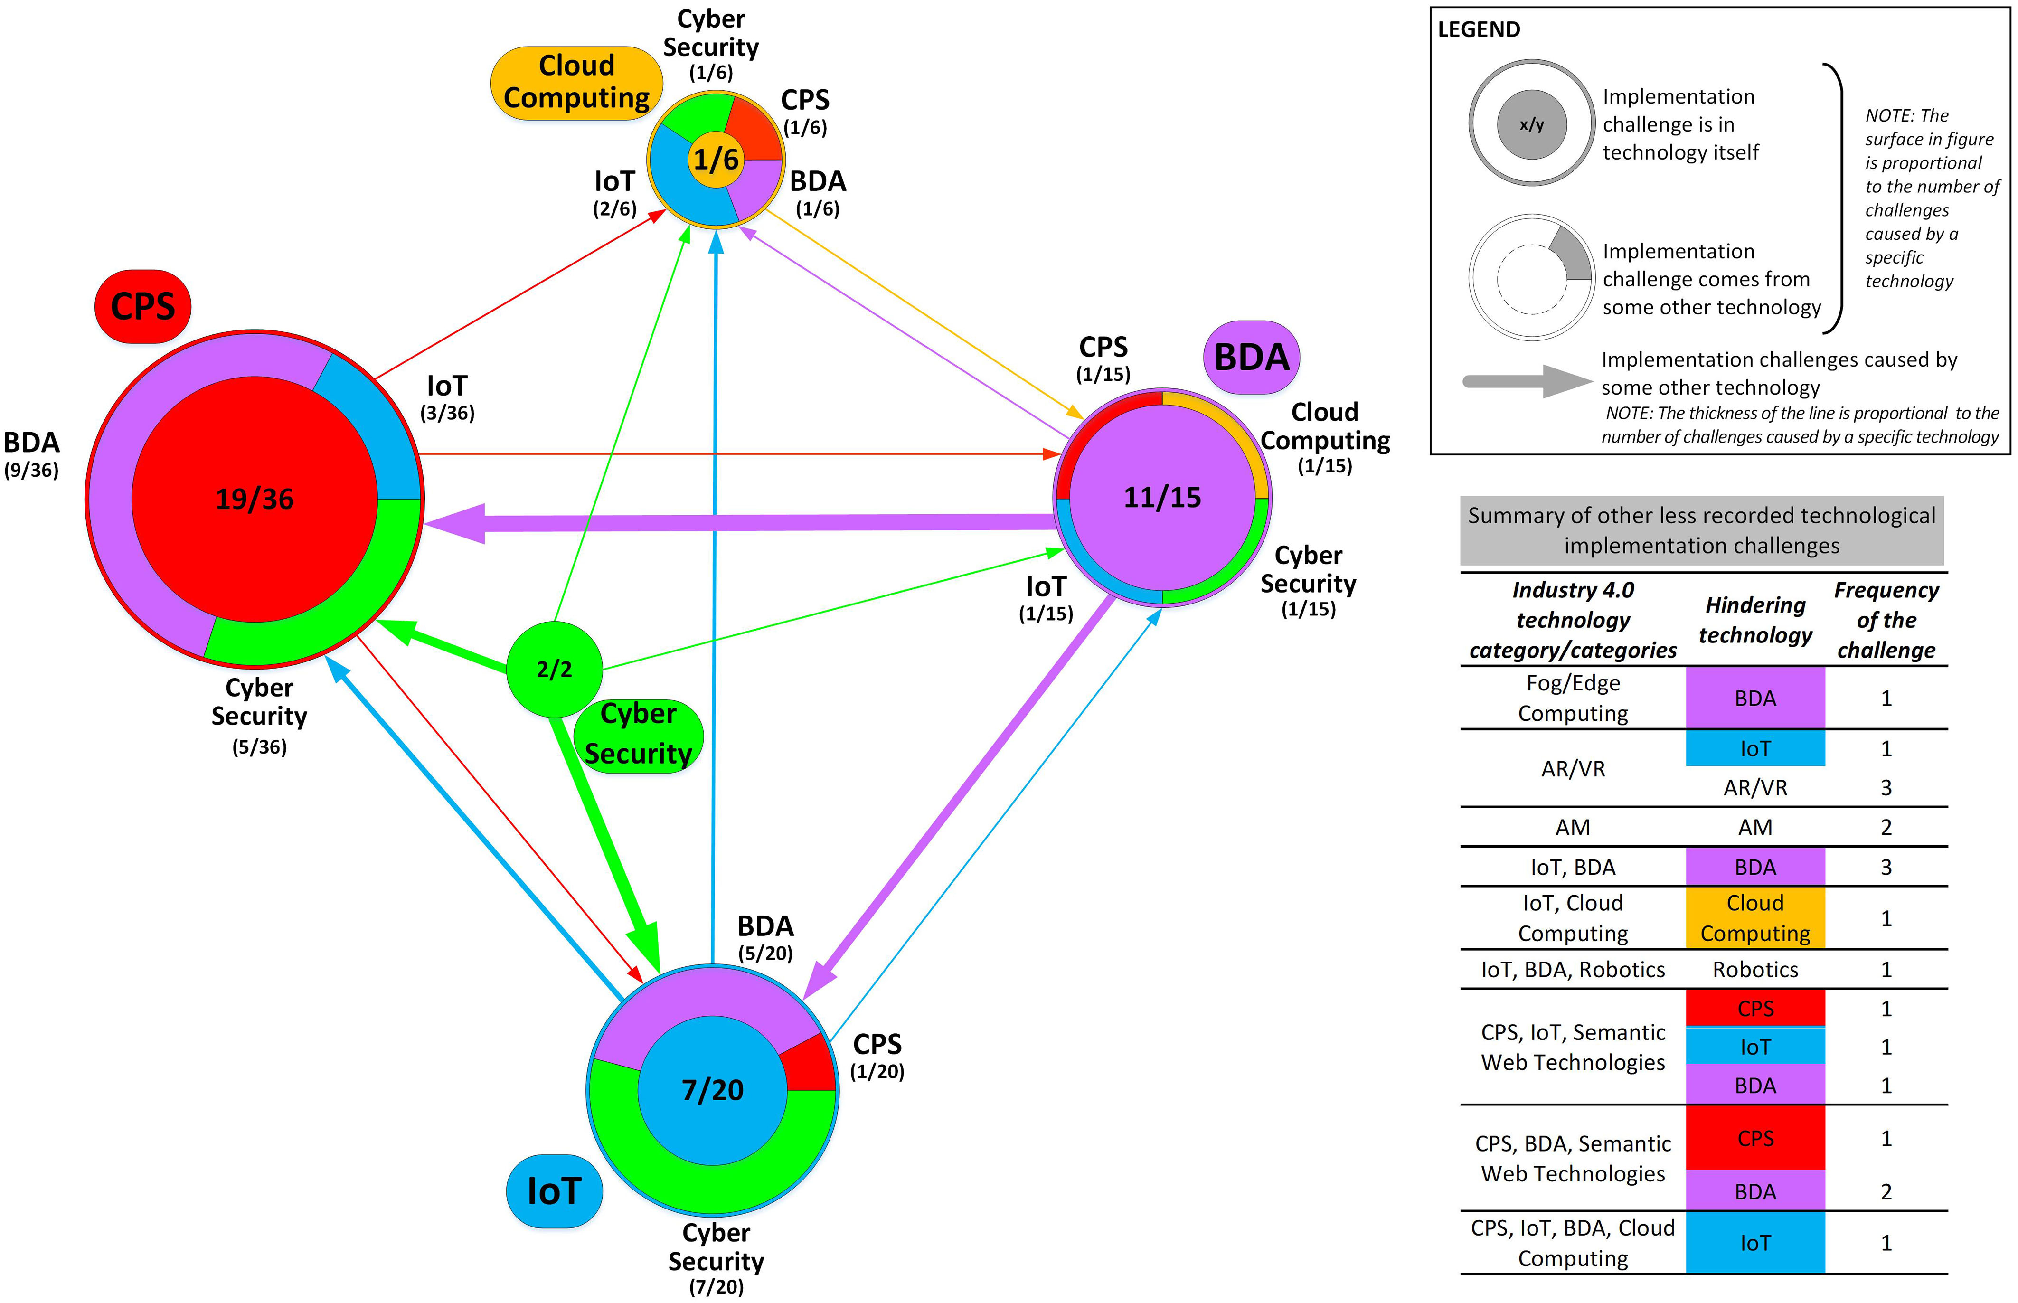
\includegraphics[scale=0.95]{images/Related/chalanges.png}
    \caption{The image portrays the frequency of challenges associated with the implementation of Industry 4.0 by technological areas. For the formation of this image, 47 of the 67 most relevant articles were used on technological problems in the implementation of technologies linked to this new industry model. Source: \cite{Rikalovic2022}.}

    \label{fig:serp}
\end{figure}

Uma dos desafios é a necessidade de melhora da segurança cibernética. A presença de vários dispositivos interligados a uma rede interna ou externa traz várias preocupações de segurança, tendo em vista que linhas de fábrica podem ser vitimas de ataques "hackers", o que compromete a funcionalidade de uma linha de produção ou o vazamento de dados sensíveis \cite{Gilchrist2016}.  Uma das formas para mitigar problemas de segurança é o uso de um sistema de authenticação BSeIn, o qual é construido em cima da tecnologia de blockchain pelos autores \textcite{LIN201842}. Além disso, outro desafio é a criptografia da comunicação entre os \acrshort{cps} em uma rede inustrial, os autores \textcite{Kreiser2018} relatma formas de criação e comunicação de chaves de criptografia em um ambiente controlado que simula uma linha de manufatura. No entanto, a forma de aplicar as medidas de segurança ficam limitadas as capacidades de implementação delas, aos recursos disponíveis e ao problema abordado. 

Outro desafio relatado pelos autores \textcite{PENAS201752} é a dificuldade de integração do meio virtual com o físico. Pois, geralmente, os \acrshort{cps}  empregam o uso de sensores, unidades de processamento e atuadores no seu funcionamento. Além da necessidade de conhecimento do gerenciamento de cada  \acrshort{cps}, é necessário saber como cada uma dessas unidades se comunicam entre si em um ambiente de larga escala de forma que esssa possam se adaptar a condições imprevistas. Outro problema é a a falta de compatilidade entre espaços reais e espaços virtuais, tendo em vista que as simulações são relaizadas em um meio discreto o que pode ser fonte de incerteza e precisão \cite{Rikalovic2022}. Além disso, a dificuldade da sincronização de um \emph{digital twin} é um desafio para a implementação dos \acrshort{cps}. Pois é necessário que o modelo virtual esteja em sincronia com o físico para que esse responda corretamente as ações produzidas pelo ambiente externo a sua volta. A falta de alta fidelidade e sincronização um enorme desafio para que os \acrshort{cps} funcionem da forma planejada \cite{Zhang2017}. 

A adaptação de sistemas existentes a nova metodologia é um enorme desafio. A falta de treinamento e capacitação dos trabalhadores uma barreira  para a modernização, pois as novas tecnologias requerem uma reciclagem do aprendizado de funcionários que pode estar a realizar a mesma função há anos. E isso pode representar um investimento significativo para as empresas, especialmente as pequenas e médias além de resistências a mudanças. 

Sem falar, na necessidade da integração dos equipamentos e sistemas antigos com as novas tecnologias. O que pode requerer a atualização de componentes obsoletos ou a adaptação dos sistemas para garantir a compatibilidade. Isso pode representar um investimento significativo para as empresas, especialmente as pequenas e médias. 

A falta de maturidade das tecnologias envolvidas desafia a implantação e a confiabilidade delas na indústria. Os autores \textcite{Rikalovic2022} relatam que os \acrshort{cps} não possuem uma tecnologia amplamente implementada, poucos softwares disponíveis e problemas de delay de comunicação. Sem falar que outras tecnologias que as \emph{"smart factories"} utilizam como: \acrfull{vr} e \acrfull{bda} aidna precisam se desenvolver muito mais para serem confiáveis na sua empregabilidade.

Em resumo, essas abordagens voltadas para TI (Tecnologia da Informação) na indústria apresentam uma possível melhoria do processo de manufatura. O modelo de Industria 4.0 é uma tendência que visa promover uma revolução industrial voltada para a utilização de tecnologias de pontas para o aumento da performance de produção. Essa abordagem permite que as linhas de produção sejam mais maleáveis tanto para produzir produtos com características diferentes quanto para responder de forma mais rápida a imprevistos que ocorram durante a manufatura. Ou seja, é possível que os \acrshort{cps} tomam decisões de forma autônoma ou não tanto a imprevistos quanto a mudanças estratégicas de produção. Além disso, esse novo modelo industrial traz atona produtos inteligentes que conversam com a linha de produção e permite a obtenção de informações sobre seu estado, o que pode ajudar a prever falhas ou melhorar a satisfação do cliente e ter um impacto  positivo na cadeia de valor do produto \cite{economies6030046}.  No entanto, toda essas tecnologias envolvidas trazem dificuldades de implementação, seja por questões que envolvem recursos financeiros, conhecimento, segurança, aceitação, adaptação ou maturidade das tecnologias.  




\section{Digital Twin}
\label{sec:digitalTwin}


O conceito de \acrfull{dt} tem usa idéia central no ano de 2003 \cite{Mihai2022, Barricelli2019}. Os autores \textcite{Grieves2017} realizaram uma apresentação  na universidade do Michigan, sobre o tema \textit{“Conceptual Ideal for Product Lifecycle Management”}, na qual a figura \ref{fig:digitalTwin} foi utilizada.  Os autores relatam que apesar de a apresentação inicial ser caracterizada como uma técnica de gerenciamento de produto, essa já trazia em si todos os elementos do que viria a ser a definição de \acrlong{dt}.

\begin{figure}[h!]
    \centering
    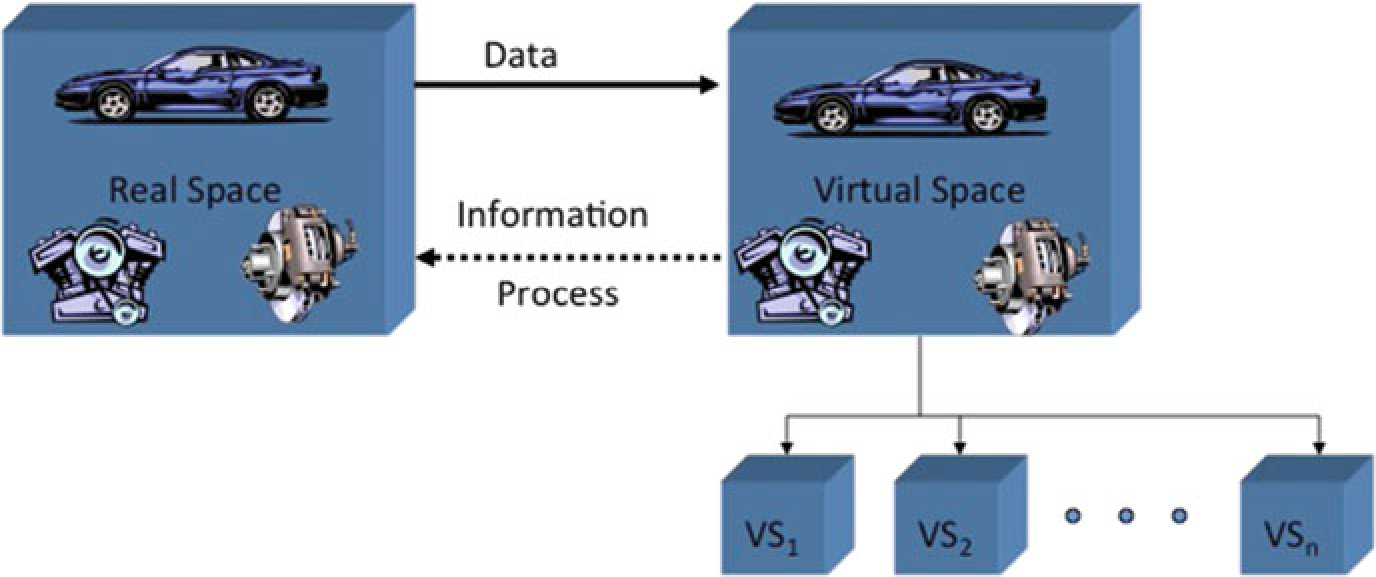
\includegraphics[scale=0.5]{images/Related/digitalTwing.png}
    \caption{Conceptual ideal for PLM. Dr. Michael Grieves, University of Michigan, Lurie Engineering Center, Dec 3, 2002. Source: \cite{Grieves2017}.}

    \label{fig:digitalTwin}
\end{figure}

Um \acrfull{dt} é uma máquina ou modelo baseado em computador que imita, emula, espelha a vida de uma entidade física. Prediz continuamente os estados futuros e permite simular e testar novas configurações, de forma a aplicar preventivamente as operações de manutenção preventiva \cite{Barricelli2019}. Segundo  \textcite{Mihai2022} tal definição corrobora com a previamente criada pelos autores \textcite{Grieves2017}.  De fato, nesse caso o conceito se permanece preservado. No entanto, o conceito de \acrshort{dt} ganhou popularidade em vários setores e outros autores buscaram evoluir sua definição ao longo do tempo, incorporando tecnologias como \acrshort{ai}, aprendizado de máquina,  \acrshort{iot}  entre outras. 

Os autores \textcite{Grieves2017} propõem que o conceito \acrfull{dt} consiste em dois sistemas: o sistema físico que sempre existiu e um novo sistema virtual que contém todas as informações sobre o sistema físico. O sistema virtual é usado para modelar e simular o sistema físico no espaço virtual, permitindo entender melhor a forma emergente e os comportamentos do sistema. Ou seja, a parte virtual do sistema pode permitir a realização de diversas simulações em $N$ diferentes espaços virtuais $VS_n$, de forma a permitir entender como o sistema se comporta nesses diferentes possíveis ambientes. Isso ajuda a reduzir o fator “eu não esperava por isso”.

De forma simples, \acrlong{dt} é um sistema de sistemas. Basicamente, \acrshort{dt} é um sistema que permite obter dados providos de diferentes tecnologias e contextualizar toda essa informação em uma representação virtual sobre um objecto e como ele interage com outros elementos ao seu redor. Ou seja, um sistema de sistemas de tecnologia que permite replicar elementos, processos, dinâmica e firmware de um sistema físico em um equivalente digital \cite{Mihai2022}. Por exemplo, o author \textcite{Mendi2022} relata um estudo de caso em uma linha de produção automotiva na Turquia. Nesse estudo, o autor coletou dados específicos de máquinas e aplicou técnicas de \acrfull{ml} para  a analise dos dados obtidos.  Isso permitiu que simulações fossem executadas para identificar possíveis problemas antes do início da produção real, além de fornecer informações sobre como a tecnologia de \acrlong{dt} poderia melhorar a eficiência e reduzir o tempo de inatividade dessa fábrica em particular. Dessa forma é possível perceber que \acrlong{dt} é um sistema que envolve outras tecnologias para a obtenção de um modelo virtual que tenta representar da melhor forma possível um objeto de estudo real. A figura \ref{fig:digitalTwinTree} tenta retaratar essa idéia. 
\begin{figure}[h!]
    \centering
    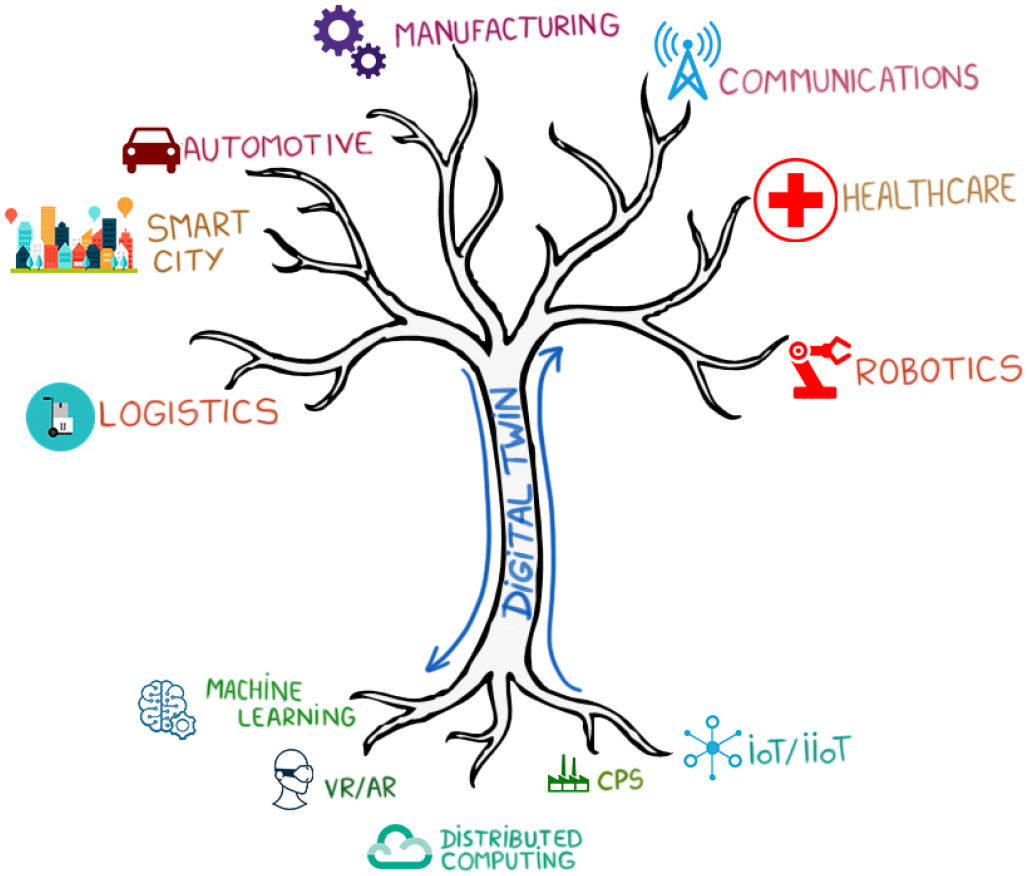
\includegraphics[scale=0.75]{images/Related/DTTree.png}
    \caption{The Digital Twin’s central role in the Industry 4.0 era. Source: \cite{Mihai2022}.}

    \label{fig:digitalTwinTree}
\end{figure}

Existem dois tipos de\acrlong{dt}: \acrlong{dtp} e digital \acrlong{dti}. O \acrshort{dtp} descreve o protótipo do objeto físico e contém os conjuntos de informações necessários para descrever e produzir uma versão física prototípica capaz de produzir uma versão virtual.  Esses conjuntos de informações incluem Modelo 3D totalmente anotado, Lista de Materiais (com especificações de material), Lista de Processos, Lista de Serviços, Simulações numéricas e etc.  O \acrshort{dti}  é um conceito que descreve um produto físico que possui um gêmeo virtual atrelado a esse durante boa parte do seu ciclo de vida. Dependendo dos casos de uso necessários, esse tipo de Gêmeo Digital pode conter, mas não está limitado aos seguintes conjuntos de informações: Um modelo 3D totalmente anotado com Dimensionamento e tolerância geométrica que descreve a geometria da instância física e seus componentes, uma lista de materiais que lista os componentes atuais e todos os componentes anteriores, uma lista de processos que lista as operações que foram executadas na criação desta instância física, juntamente com os resultados de quaisquer medições e testes na instância, um registro de serviço que descreve serviços passados executados e componentes substituídos, e estados operacionais capturados a partir de dados reais do sensor, atuais, passados reais e futuros previstos \cite{Grieves2017}. 

  

O modelo \acrshort{dtp}  é uma oportunidade para identificar e eliminar situações imprevistas e indesejáveis \cite{Grieves2017}. Esse tipo de conceito permite que as pessoas envolvidas no projeto utilizem modelos 3D criados em softwares de \acrfull{cad} e \acrfull{cam}, que permitem visualizar e testar virtualmente suas ideias em um ambiente simulado. Além disso, o uso de simulações numéricas como \acrfull{fem}, \acrfull{bda} entre outras também é comum no processo de design, permitindo a análise de como o produto ou sistema se comportará em diferentes condições e sob diferentes cargas. Dessa forma, os projetistas podem prever possíveis causas de falha do seu produto como: falha por estresse da estrutura, problemas de aerodinâmica, problemas de criação de circuitos eletrônicos, erros de comunicação entre as tecnologias previstas, lista de materiais necessárias e etc. Com essa prototipação inicial definida é possível prever uma série de falhas e erros de concepção de projeto evitando assim gastos desnecessários com a construção de protótipos ou, no pior dos casos, do produto real a qual não teria a performance requerida. 

  

Porém vale apena ressaltar que \acrshort{dt} não pode ser resumido simplesmente a um software \acrshort{cad} \cite{Barricelli2019}.  Para um sistema ser considerado um \acrshort{dt}, precisa-se de três blocos funcionais, esses são: um ativo físico, uma contraparte virtual e um sistema de comunicação que permita a comunicação entre esses blocos. Tal meio de comunicação precisa ser um canal de fluxo de informação bidirecional, que permita tanto a saída quanto a entrada dos dados do modelo real para o virtual \cite{Mihai2022}. Dessa forma, um modelo 3D \acrshort{cad}, pode ser apenas uma das partes associadas a construção do \acrlong{dt}. 

  

  

O \acrlong{dti} permite entender, prever falhas e inúmeras outras possibilidades sobre o produto. Esse tipo de modelo virtual pode possuir uma série de informações do produto real que permitem a criação de modelos virtuais que replicam sistemas, produtos ou ativos físicos. De tal forma que esses são conectados a seus equivalentes do mundo real por meio de sensores e redes de comunicação de dados. Isso permite a análise de históricos do produto, independentemente da localização física de suas contrapartes. Os dados coletados de vários \acrshort{dti} podem ser correlacionados e analisados para prever estados futuros, ajudando a melhorar a manutenção e o desempenho dos sistemas físicos. A capacidade de interrogar \acrshort{dti} fornece informações valiosas para monitorar, prever e otimizar as operações de sistemas físicos, produtos ou ativos. Dessa forma, nesse tipo de modelo virtual um dos tópicos que vem ganhando destaque é a manutenção preventiva \cite{Grieves2017}. No entanto, essa é apenas uma de inúmeras possibilidades que esse conceito oferece. 

  

Atualmente existem alguns ramos da indústria em que há um maior destaque no desenvolvimento de aplicações relacionadas a \acrshort{dt}, esses setores são: aviação, automotivo, assistência médica e manutenção preditiva. Os avanços nessas arias se deve tanto pela potencialidade de melhorias quanto a importância dessas áreas, seja financeira ou humana. Por exemplo, a indústria aeronáutica possui grande interesso no constante monitoramento das aeronaves para evitar danos materiais ou acidentes com prejuízo à vida humana. Para o caso da manutenção preditiva, pode-se observar também que além da importância financeira, os avanços recentes tecnológicos permitem que esse ramo se torne cada vez mais prático. Atualmente, há enormes avanços em desenvolvimento de técnicas e algoritmos para a predição de possíveis pontos de falha. Assim, essas áreas permitem um grande avanço prático tanto pela justificativa de importância de solução de possíveis problemas quanto pela disponibilidade recente de tecnologias que permitem que isso seja possível.  


Atualmente existem alguns ramos da indústria em que há um maior destaque no desenvolvimento de aplicações relacionadas a \acrshort{dt} , esses setores são: aviação, automotivo, assistência médica e manutenção preditiva. Os avanços nessas áreas se devem tanto pela potencialidade de melhorias quanto a importância dessas áreas, seja na parte financeira ou humana. Por exemplo, a indústria aeronáutica possui grande interesso no constante monitoramento das aeronaves para evitar danos materiais ou acidentes com prejuízos à vida humana. Para o caso da manutenção preditiva, pode-se observar também que além da importância financeira, os avanços recentes tecnológicos permitem que esse ramo se torne cada vez mais prático. Atualmente, há enormes avanços em desenvolvimento de técnicas e algoritmos para a predição de possíveis pontos de falha, como o uso de \acrfull{ann} \cite{He2019PreliminaryEO}. Assim, essas áreas permitem um grande avanço prático tanto pela justificativa de importância de solução de possíveis problemas quanto pela disponibilidade recente de tecnologias que permitem que isso seja possível. 

O uso de \acrshort{dt} na manufatura pode prover uma melhora na eficiência dos processos, por meio de uma automatização de tarefas e no suporte da tomada de decisões \cite{ROSEN2015567}.
Os autores \textcite{Qi2018} também relatam que o uso de \acrfull{bd} permite ao \acrshort{dt} obter uma melhoria da eficiência dos processos e previsões sobre dados coletados ao longo da linha de manufatura. Por exemplo, o uso de \acrshort{bda} permite a tentativa de prever possíveis pontos de falha tanto ao longo da vida de um produto como a ocorrência de falhas em maquinários envolvidos na fabricação desse, figura \ref{fig:digitalTwinBigData}. Dessa forma, \acrshort{bda} possui grande potencial para o uso em manutenção preditiva ou para a adequação do produto a determinados padrões que satisfaçam os interesses do usuário final.  Os autores \textcite{Tao2017} exploram a idéia do uso de \acrshort{dt} para o chão de fábrica de uma linha de produção, por meio de formas de implementar o conceito. Ou seja, métodos de implementar  uma contraparte virtual da linha de produção. Dessa forma, poder analisar possíveis pontos de falhas e aplicar optimizações de layout ou de processos. Dessa forma, atualmente \acrshort{dt} passa a ser cada vez mais usado em fábricas para melhorar processo e produtos.

No ramo aeronáutico o uso de \acrshort{dt} é utilizado mais para a área preditiva, ou seja, detectar o surgimento de possíveis pontos de falha e acionar sistemas de mitigação \cite{Barricelli2019}. Por meio de métodos estatísticos e com abordagens numéricas envolvendo sistemas  multi-físicos é possível estimar possíveis falhas na aeronave através de dados iniciais de entrada \cite{Benjamin2012}. Um exemplo é o caso em que os autores \textcite{Bielefeldt2015} propõem o uso de \acrlong{fem} com \acrshort{dt} para obter possíveis pontos de falha em uma asa de um avião comercial. Dessa forma, atualmente, o uso de \acrshort{dt} possui um papel importante na previsão de possíveis imprevistos ou falhas que venham ocorrer em uma aeronave, o que pode provocar enormes danos materiais e a vida humana. Com a presença de um sistema que possa de forma prévia detectar possíveis erros é possível mitigar essas ocorrências ou solucioná-las com estratégias ou técnicas de correção e segurança. 

\begin{figure}[h!]
    \centering
    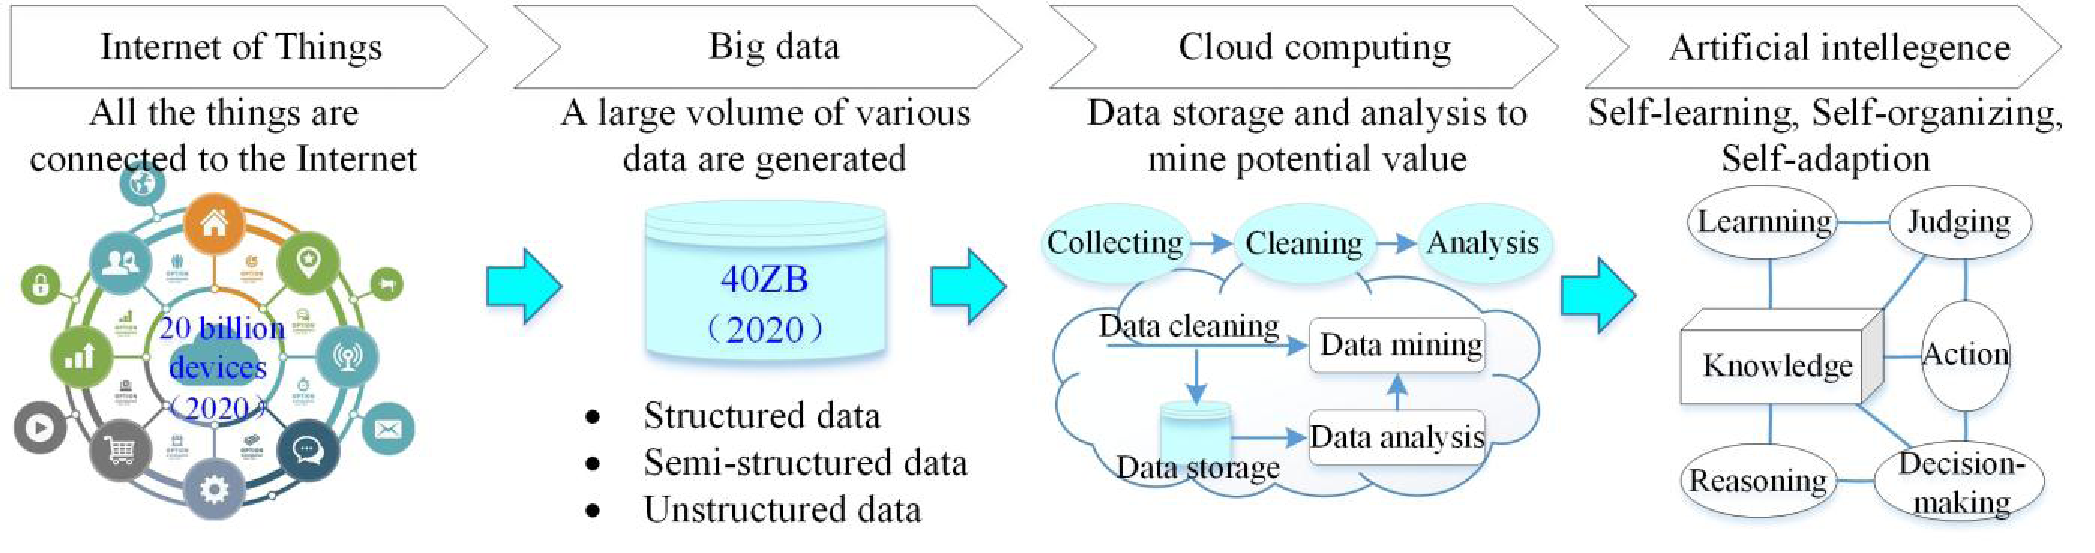
\includegraphics[scale=0.75]{images/Related/cps.png}
    \caption{formation of the life cycle of a product through the use of cybernetic physical systems. Source: \cite{Qi2018}.}

    \label{fig:digitalTwinBigData}
\end{figure}

Recentemente, a área de assistência média  é outro ramo que vem obtendo grandes avanços na implementação de novas tecnologias e técnicas. \acrlong{dt} é um dos novos conceitos sendo implementado na área da saúde com o objetivo de criar um sistema virtual do corpo humano ou de seus órgãos  para que seja  atingir o objetivo de prever possíveis doenças ou maus funcionamentos do corpo humano, além de gerenciamento da disponibilidade de bens de um hospital. O  \textcite{johns_2016} fez o uso de \acrshort{ann} para realizar simulações e tomar as melhores decisões possíveis de gerenciamento dos seus recursos, o que é crucial para salvar vidas. Outro caso foi o uso de um \acrshort{dt} pela Siemens Healthineers no hospital Mater Private Hospitals (MPH) em Dublin \cite{gilligan_digital_2018}. Nesse estudo de caso o hospital apresentava falta de espaço, leitos, atrasos e alta demanda de pacientes. Para resolver esses problemas, Siemens Healthineers redesenhou o departamento de radiologia com o desenvolvimento de uma \acrshort{ann} para gerenciar o departamento e suas operações. Com isso, obteve-se um \acrshort{dt} do departamento, permitindo a realização de simulações para achar um layout opitimo e um controle e monitoramento das tarefas. Outro exemplo de \acrfull{dt} é o projeto \emph{The Living Heart} \cite{Levine2022}, figura \ref{fig:digitalTwinHeart}, esse projeto permite que cientistas simulem o coração humano. Permitindo que seja relizado uma simulação verossímil e multifásica, que toma  vários campos físicos como: eletromagnética, fluidodinâmica e mecânica. Dessa forma, cientistas podem usar essa ferramenta para auxiliar estudos de como determinados stresses físicos ou doenças cardiovasculares podem impactar o funcionamento desse órgão. 

\begin{figure}[h!]
    \centering
    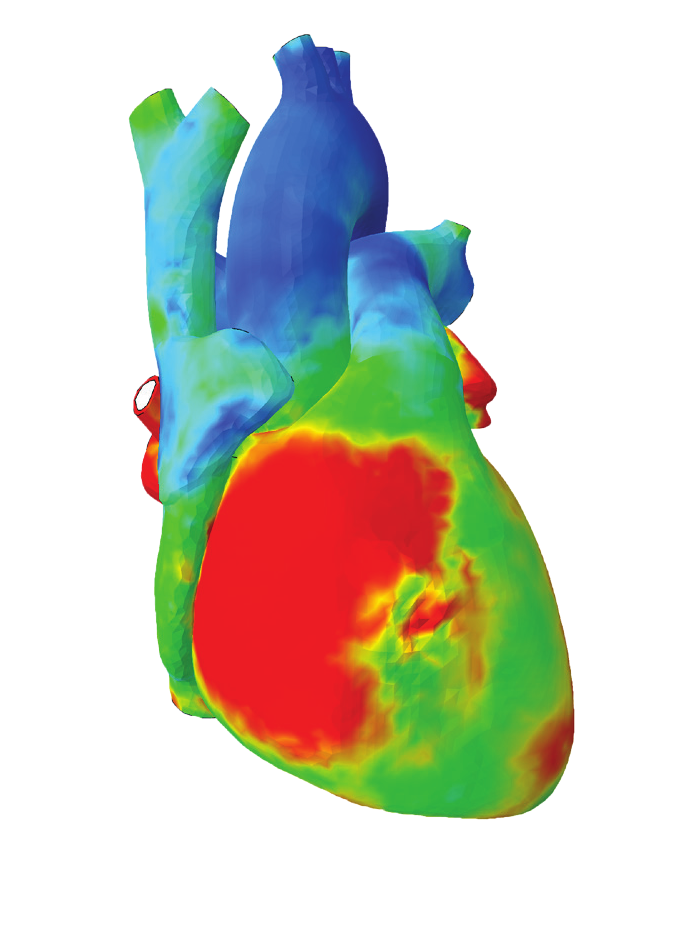
\includegraphics[scale=0.75]{images/Related/heart.png}
    \caption{Stresses  simulation depicted on a 3D rendering of the Living Heart Model. Source: \cite{Levine2022}.}

    \label{fig:digitalTwinHeart}
\end{figure}


Em resumo, o conceito de \acrfull{dt} permaneceu bastante estável desde sua criação em 2002 passando por adaptações frente as mudanças tecnológicas que foram aparecendo. \acrshort{dt} é formado por duas partes: o sistema físico e o sistema virtual. A função do \acrshort{dt} é e contextualiza dados de diferentes tecnologias em uma representação virtual de um objeto e como ele interage com seu entorno. Dessa forma, várias tecnologias podem ser integradas nesse sistema como: \acrlong{ann}, \acrlong{bda}, \acrlong{iot}, \acrlong{vr}, \acrlong{vr} entre outras. Com esses dados gerados e processados é possível obter dados sobre: possíveis futuras falhas, informações de localização, estado físico atual, interesses do usuário final sobre o produto e etc. De forma geral, \acrshort{dt} faz parte da nova revolução industrial com enorme potencial de reduzir custos e aumentar a produtividade de linhas de produção, além de possibilitar que o produto final tenha uma vida maior e seja mais seguro. 



\section{IoT Architecture}

As the \gls{IoT} systems are gaining popularity, it becomes important to understand the basic about their structure and which tasks and functions each of the layers are responsible. Despite the fact there are some divergence in literature about the structure of the \gls{IoT}, normally it is made-up by three layers namely as Perception, Network and Application layers \cite{SWAMY:2017}. 

The first layer called Perception, also known as "Sensors", is responsible for collecting the information from the environment using sensors. There are many different types of sensors that perform variety of tasks, e.g., level measurement, proximity, temperature, humidity, accelerometers, gyroscope, etc, which can be used in many useful applications \cite{ALOTAIBI:2016}. Thereby, the gathered data by sensors are  transmitted to the Network layer. 

The Network layer consists of communication networks and communication protocols responsible for Routing and Transmitting the data to different \gls{IoT} hubs and devices over the Internet. It uses different communications technologies such as Wi-Fi, Bluetooth, 3G network, Long-Term Evolution (LTE), etc. As approached by \cite{SWAMY:2017}, it also takes place the Data aggregation, Data filtering and transmission.

The last one is the Application layer, which is subjected to provide the Data Integrity, Data confidentiality and Data authenticity, carrying out application specific functionalities. In some architecture it is divided in two parts: Firstly, the business layer which is responsible for application management and security and privacy issues; The second one, also known as application layer, being responsible for distinguishes among different applications \cite{TEWARI:2018}. 


\section{Web Development applied to IoT}

The advancements of \gls{IoT} systems will have several impacts in the world of business \cite{TURC:2019}. The use of \gls{TCP} is on focus to have extensive deployment, allowing the \gls{IoT} sensor nodes to send information directly to servers and users through Internet protocols \cite{HART:2015}.

The management of the data collected by the \gls{IoT} device, as also approached in this work, uses the Web technologies in order to maintain the website functionality. The client-side/server-side and database technology connection is required as part of the hierarchy for transferring data and enabling the communication with the user \cite{WEBDEVELOPMENT:2019, AGGARWAL:2019}. A recent researched was proposed at the 12th International Conference Interdisciplinarity in Engineering in which \gls{AJAX} technology is used in the context of \gls{IoT} \cite{TURC:2019}. The work relies on the server-client paradigm, which the data collected by the \gls{IoT} device is managed by the server-side, stored in the database and it responds to the client's continuous requests via \gls{AJAX}. The adoption of \gls{AJAX} as web-based application provides intuitive information and interaction, allowing the data to be stored and dynamic accessed by the client. 

Another factor that is important is that the integration of Web development in \gls{IoT} concentrates more on the system's scalability and security than conventional Web development \cite{AGGARWAL:2019}. In 2017, \cite{ZIEGLER:2017} presented an analytical perspective about the network scalability for addressing the \gls{IoT} exponentially growing. The work intended to provide some new perspectives about the \gls{IPv6}, considered to be one of the strongest candidate in terms of network protocol. The work exposed an extended scale of the address structure of the \gls{IPv6}, in order of magnitude and large scale numbers, which made possible to assess its potential. It is demonstrated that the \gls{IPv6} addressing capacity is widely enough to meet all the present and future necessities of human-to-human and machine-to-machine at the scale of mankind.

A recent survey made by the Eclipse Foundation \cite{ECLIPSE-SURVEY:2019} revealed that 49~\% of the participants use \gls{HTML} as a communication protocol, followed by 42~\% using Message Queuing Telemetry Transport (MQTT) and 26~\% using websockets. Also, the survey reported that 54.1~\% of the participants uses the \gls{TCP}/\gls{IP} as a connectivity protocols. These information are used to gain a better understanding of the requirements, priorities and perceptions that the \gls{IoT} developers are having, demonstrating the path the \gls{IoT} system is having through the web development industry. 


\section{Methods used in Level Measurement Systems}


The level parameter is not a new term and it represents an important indicator for process control to know how much raw material there is in stock, how much material is in the manufacturing process and how much of final product is ready for the market \cite{SA:2001}. Due to the purpose of the work, this chapter introduces a brief idea about the gamma of possibilities of determining the level of liquids in vessels and storage tanks.

In 2004, \cite{BOLTON:2004} exemplifies some methods to measure the level of liquids in vessels. Different methods can be used, e.g., floating position, Archimedes' principle, differential pressure, load cell, electrical conductivity level indicator, capacitive level indicator, ultrasonic and nuclear radiation. Although each method presented has its own principle and technique of operation, the advantages and disadvantages when applying for a specific function must be studied in order to have a better performance evaluation, as demonstrated by a research in which it was used water as the monitored material \cite{LOIZOU:2016}. 

In 2016, \cite{LOIZOU:2016} presented a review of techniques applicable for monitoring water level, in a relative low range, and proposes a method using capacitive-type sensor. The review address solutions using capacitive-type sensors such as cylindrical capacitive sensors or even different versions of capacitive-type sensors, although it shows low cost, easy installation and high linearity characteristics, it also has shown some concerns about the high level of humidity which can be created inside of the tank, compromising the electrodes that compose a capacitive sensor, when it is not made up of stainless steel type. Another type analysed by \cite{LOIZOU:2016} is the optical sensing techniques, which may extend the applications to dangerous chemical liquids, but it shows high sensitivity to temperature variation. Others methods approached by the study are the microwave radars, used in both marine and non-marine environments, ultrasound sensor and a signal processing technique using Time-Domain Reflectometry (TDR). This type of method is widely used for liquid monitoring which requires electrodes immersed into the liquid. 

The investigation of a novel capacitive-type water level measurement, as proposed by \cite{LOIZOU:2015}, has shown operation characteristics and performance, through simulations and experimental tests, conducted in two water storage tanks, with a city-scale water distribution network. The comparison made, with existing industrial water-level monitoring systems, has demonstrated that the study comprises a competitive alternative for incorporation in water management systems.

A recent research has proposed a new water level sensor using a load cell and a enclosing floating pipe \cite{WANG:2018}. 
The idea is to perform a contact water-level-technique with an extend lifetime. In order to have a more precise sensing technique than the non-contact method, it was used an enclosing floating pipe responsible for making the link between the liquid and the load cell, which is the key sensing element. The result from the preliminary study of the indirect measurement has shown feasibility, however the solutions to solve the impacts of fluctuations caused by the water flows are still being analysed and studied.

Another study has addressed the level measurement techniques through the use of Radar Sensors in Industrial Process \cite{VOGT:2018}. The study analysed some technological aspects of frequency-modulated continuous-wave (FMCW) concept of radar level meters and, over comparisons between the 24 GHz and 80 GHz frequency ranges, the 80 GHz level radars offer a better Signal-to-noise Ratio (SNR) over the 24 Ghz in general, which has shown better results only in special cases. 

Therefore, there are a large gamma of possibilities for level measurement systems that can be used. Thereby, next section will approach techniques for level measurement using ultrasonic sensing methods.


\section{Ultrasonic Sensing Methods for Level Measurement Systems}\label{ultrasonic sensing methods}

The ultrasonic sensor is a widely used technology in which its application have a large range of possibilities. The principle of work is similar to radar or sonar which evaluate attributes of a target by interpreting the echoes from radio or sound waves respectively. This technology can be used in robotics barrier, object distance measurement, security systems, vehicle detection/avoidance, level detection, etc \cite{datasheet:US015}. 

In 1994, \cite{LONGBOTTOM:1994} proposed a new technique with ultrasonic sensor used in solid level measurements, as the technology was already well established for liquid level measurements in the industrial process. Due to the variations in the shape of a solid surface, the idea of the project was to use a single emitter with multiple receiver in order to pick-up the distortions and directional returning waves, then the signals may be processed appropriately for improvements in reliability and accuracy. Through simulations techniques being used with all the relevant information modelled mathematically, the research verify that the result from the method can illustrate errors up to 60~\%, suggesting that further improvements still need to be made.

Already in 2004, researchers developed a Multi-layer Level Measurement for monitoring the propagation of ultrasonic waves in the oil, water and mixed oil-water liquids \cite{MERIBOUT:2004}. The idea of the project was based on that the amount of ultrasound waves received and the speed dependency of the liquid density. Through the vertical layout of the measurements of the signal response, the level detection of the two interface is made. Thus, extensive experiments was made in five consecutive steps, with the device developed, and some positive results were taken, showing a certain viability of the work. 

A similar study, approached by \cite{LEE:2005}, was presented in the next year, however, differently than the first one, the ultrasonic method now is responsible to measure the two-phase mixture level with the application to a nuclear reactor or steam generator during abnormal conditions as well as normal conditions. The development of the work demonstrated that, the method accurately measures the two-phase mixture using the correction formula, as approached by the study. Also, in order to reduce the loss of echo by the effects of attenuation, the waveguide developed effectively measures the level of the fluid more accurately than the conventional ultrasonic methods, at high temperature and high pressure environment.

In 2006, it was developed a method to measure the air conditioning compressor used in the passenger train car, in China, using the ultrasound method \cite{CHEN:2006}. As approached by the study, most of the breakdown was caused because of the refrigerant oil in the container was reduced to a level under the definite line. Thereby, the transmitting and receiving circuit was designed and a software was developed, allowing the ultrasound signals to be analyzed at real time with the use of a computer. The study provided an effective method for the liquid measurement and, because of its modular structure as addressed at the work, the instrument can be easily transplanted to other relative fields, presenting a large potential for the integrated systems advancements.

Other advances were made by researchers in which they evaluated the level measurements from the ultrasonic sensors by means of the Wavelet Transform. The concept idea is based on the \gls{ToF} technique, which is the time difference between the instant the ultrasonic signal is emitted to the instant when the ultrasonic signal is detected. Also, there is an uncertainty of the measurement originated by the attenuation, additive noise and multiplicative noise of the signal. As approached by the researchers, in order to calculate the levels with low uncertainty measurements, the Wavelet Transform is chosen because it decomposes the signals using filter banks, becoming possible to obtain a representation of the ultrasonic echoes with low noise level. Both of the studies demonstrated that the wavelet threshold technique is very reliable, being possible to estimate the distances with a good approximation to the theoretical values, even under severe noise conditions \cite{INGAROCA:2011, GRASSI:2014}.  

In 2015, \cite{LI:2015} proposed a new method for improvement the measuring accuracy of dynamic liquid level case. The study approached some new relevant findings in radar technology and proposed a distinctive liquid-level measurement that is based on the Multiple-input Multiple-output (MIMO) ultrasonic transducer array, thereby allowing it to achieve the reduction of system complexity and cost, and also making it possible to acquire rapid high precise samples of the level. The research development is composed of some relevant parts focused on the transducer array, signal transmitting and receiving channels, and signal processing unit. Moreover, \cite{LI:2015} also proposed a simulation method of ultrasonic echo signal from liquid level based on the boundary-layer theory and the ultrasonic scattering theory. Thus, the method is verified by simulation and real system, the result indicates the method can present a higher accuracy in dynamically changed liquid-level case than the conventional approach. Furthermore, the study also indicates that the focus in beamforming is properly set in every scanning direction, keeping the noise of the echo signal effectively controlled.

In 2019, \cite{ROCCHI:2019} proposed a characterization and optimization of the water level measurement in the marine environment context. The research was suggested in order to estimate the position of the water surface in order to determine the thickness and depth of the pollutant layer (hydrocarbons floating in the sea). The use of a low-cost SRF05 ultrasonic sensor is also provided by the research and the intention is to acquire a final device managed to have a sensibility of about 1 mm. The characterization was made in a close measurement range to its operating limit, with the envelope signal and Hilbert Transform methods being used in order to reduce the error of \gls{ToF}s measurements. \cite{ROCCHI:2019} suggests the use of another SRF05 sensor due to the systematic occurrence of jitter time anomaly (anomalies in the \gls{ToF} values). Also, the use of another sensor will allow to extend the operative measurement interval while preserving high accuracy measures, enabling it to avoid the need of signal post-processing, in which it will result in a reliable and accurate real-time monitoring of the surface level of the material. 